One obtains Friedmann equations by $\delta \bigintsss d^4x\sqrt{\abs{g}}\left(\frac{R}{16\pi G}+\mathcal{L}_{m}(\psi,g_{\mu\nu})\right)= 0$, with the metric being the FRW one:
\begin{equation}
ds^2_{\text{FRW}} =  dt^2 - a^2(t) \left[ \frac{dr^2}{1 - k r^2} + d\Omega^2 \right]
\end{equation}
\begin{align}
    G^0_0 &= 8 \pi G T^0_0 \quad \Rightarrow \quad \textcolor{purple!50!blue}{H^2 = \frac{8 \pi G}{3} \rho - \frac{k}{a^2} \label{00}}
    \\G^i_i &= 8 \pi G T^i_i \quad \Rightarrow \quad \textcolor{purple!50!blue}{3 H^2 + 2 \dot{H} = -8 \pi G P - \frac{k}{a^2} \label{11}}
\end{align}
Combining~\eqref{00} and~\eqref{11}, or just by imposing covariant conservation of $T^\mu_\nu$, continuity equation follows:
\begin{eqopt}
    \dot{\rho} + 3 H (\rho+P) = 0 \label{continuity}
\end{eqopt}
\begin{eqopt}[darkgreen]
    H \equiv \frac{\dot{a}}{a}   \qquad \tau \equiv \int\frac{dt}{a} \qquad a \equiv \frac{1}{1+z} \qquad a_{\text{now}} \equiv 1
\end{eqopt}
\begin{eqopt}[darkgreen]
    \omega \equiv \frac{P}{\rho} \qquad M_P^2 \equiv (8\pi G)^{-1}  \qquad \Omega_{i}\equiv \frac{8\pi G \rho_i}{3H^2} \qquad \Omega_{k}\equiv \frac{-k}{(aH)^2}
\end{eqopt}
Dust has $P=0$. For radiation one inspects the pressure components $T^{ii}=\rho/3$, as $T^{\mu\nu} = \bigintsss \frac{d^3p}{(2\pi)^3 }\frac{p^\mu p^\nu}{p^0} f(\mathbf{p})$ 
and $p^0 \equiv E = |\mathbf{p}|$ for radiation. 
Analogue for the cosmological constant: $\rho=T^{00}=\Lambda/8\pi G=-T^{ii}=-P$. Hence
\begin{eqopt}[darkred]
    \omega_m = 0 \qquad  \omega_{\gamma}=\frac{1}{3} \qquad \omega_{\Lambda}=-1
\end{eqopt}
\begin{center}
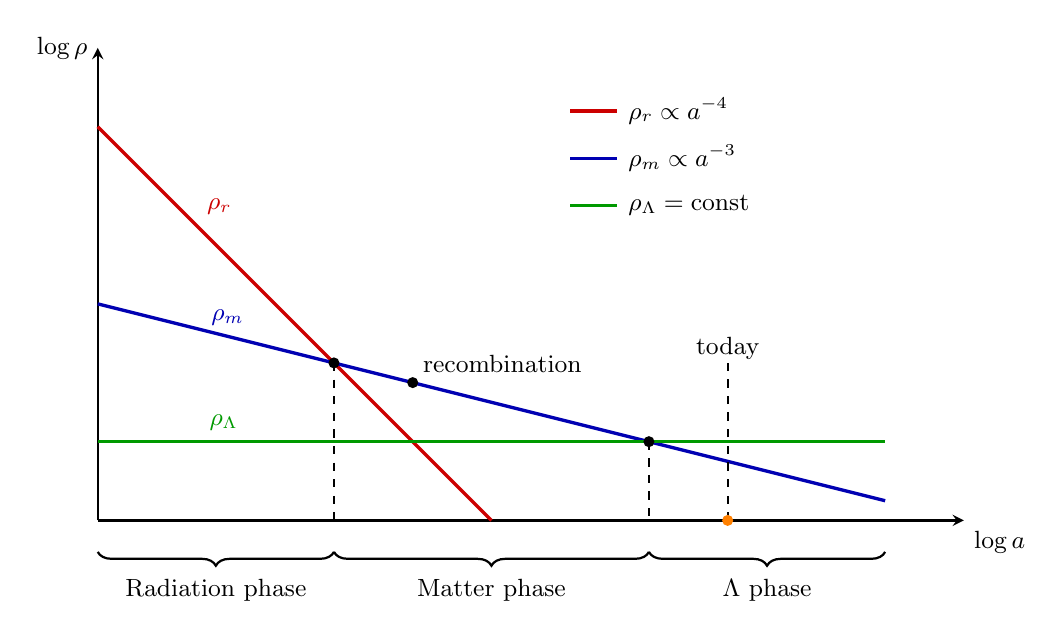
\begin{tikzpicture}[
    >=stealth,
    thick,
    font=\small,
    every node/.style={font=\small}
]

  % --- axes ------------------------------------
  \draw[->] (0,0) -- (11,0) node[below right] {$\log{a}$};
  \draw[->] (0,0) -- (0,6)  node[left] {$\log{\rho}$};

  % --- equality & recombination coordinates --------------------
  \coordinate (aeq)  at (3,2);   % matter–rad equality
  \coordinate (alam) at (7,1);   % matter–Λ equality
  \coordinate (rec) at (4,1.75);   % recombination

  % --- density curves --------------------------
  % radiation  ρ_r  (passes through (0,5) and (3,2))
  \draw[red!80!black, very thick] (0,5) -- (5,0)
      node[pos=.25,above right] {$\rho_r$};

  % matter      ρ_m  (line through (0,2.75) –> (7,1))
  \draw[blue!70!black,very thick] (0,2.75) -- (10,0.25)
  node[pos=.165,above] {$\rho_m$};

  % cosmological constant ρ_Λ
  \draw[green!60!black, very thick] (0,1) -- (10,1)
        node[pos=0.16,above] {$\rho_\Lambda$};

  % --- equality points & guides ----------------
  \fill (aeq)  circle (2pt);
  \fill (alam) circle (2pt);
  \fill (rec) circle (2pt);

  \draw[dashed] (aeq)  -- ++(0,-2);
  \draw[dashed] (alam) -- ++(0,-1);

  \draw (rec) node[above right] {recombination};

  % --- “today” marker --------------------------
  \draw[dashed] (8,0)  -- (8,2) node[above=-2.4pt] {today};
  \fill[orange] (8,0)  circle (2pt);

  % --- phase braces ----------------------------
  \draw[decorate,decoration={brace,mirror,amplitude=5pt}]
        (0,-0.4) -- (3,-0.4) node[midway,below=6pt] {Radiation phase};

  \draw[decorate,decoration={brace,mirror,amplitude=5pt}]
        (3,-0.4) -- (7,-0.4) node[midway,below=6pt] {Matter phase};

  \draw[decorate,decoration={brace,mirror,amplitude=5pt}]
        (7,-0.4) -- (10,-0.4) node[midway,below=6pt] {$\Lambda$ phase};

        % --- legend in top‐right corner ------------
  \begin{scope}[shift={(6,5)}]  % adjust (6,5) to taste
    \draw[red!80!black, very thick]   (0,0.2)   -- (0.6,0.2)   node[right, black] {$\rho_r\propto a^{-4}$};
    \draw[blue!70!black, very thick]  (0,-0.4) -- (0.6,-0.4) node[right, black] {$\rho_m\propto a^{-3}$};
    \draw[green!60!black, very thick] (0,-1) -- (0.6,-1) node[right, black] {$\rho_\Lambda=\mathrm{const}$};
  \end{scope}

\end{tikzpicture}
\end{center}
\subsection{Fine Tuning Problems in HBB}
%Horizon Problem
\begin{mycolorbox}
\textbf{Horizion problem:}

Observations tell us that the Universe is highly homogeneous and isotropic.
\begin{eqopt}[blue]
    \frac{\delta T}{T_{now}} \sim 10^{-4} - 10^{-5} \qquad T_{now} \approx 2.73 K
\end{eqopt} 
\underline{Assume $k=0$} in the metric. Rewrite~\eqref{00}~\eqref{11}. Consider a radial photon. 
Assume an initial singularity: $t_i = 0$, $a(t_i)=0$. Find \textcolor{darkgreen}{\textit{comoving particle horizon}}
\begin{equation}
    \Delta r = \int_0^t \frac{t^\prime}{a(t^\prime)} = \tau(t)-\tau(0)
\end{equation}
Use~\eqref{00}~\eqref{continuity} to relate proportionally $a$ and $t$. See that for $\omega>-1/3$ (SEC) $\Delta r$ is finite
$\Rightarrow$ \emph{there were regions not in causal contact in the past!}
Then compute the angle corresponding to the comoving horizon at recombination\footnote{Because CMB is emitted at that time! That's when the universe became transparent and photons were able to travel freely.} 
$\theta=(\tau_{rec}-\tau_{i})/(\tau_{now}-\tau_{rec})$.
Rewrite a general $\tau$ difference integrating and change variables to make $H$ appear so you can substitute with~\eqref{00}. \textcolor{blue}{$\theta \approx 1.15^\circ$}.
\end{mycolorbox}    

%Flatness Problem
\begin{mycolorbox}[red]
    \textbf{Flatness problem:}

    From current observations \textcolor{blue}{$\Omega_k <0.02$} $\Rightarrow$ one expects $\sum_i\Omega_i -1 \equiv \Omega_{tot}-1 \lesssim 10^{-2}$
    
    Compare present day to Plank epoch: 
    \begin{equation}
        \frac{\Omega_{tot}(t_{now})-1}{\Omega_{tot}(t_{P})-1} = \frac{(aH)^2|_{t_P}}{(aH)^2|_{t_{now}}}
    \end{equation}
    employ
    \begin{eqopt}[blue]
        \textcolor{darkred}{a \propto T^{-1}\footnote{Holds for radiation dominated Universe only, where $a \propto \rho^{-1/4}$ and \textcolor{darkred}{$\rho \propto T^4$ for black body radiation} }}
        \qquad H(t_P) \sim M_P \qquad T_P \sim M_P  \qquad H_{now}\sim 10^{-60}M_P 
    \end{eqopt}
    \emph{This means $\Omega_{tot}(t_P)-1 \lesssim 10^{-60}$ which would be highly fine-tuned}.
\end{mycolorbox}
